%%%%%%%%%%%%%%%%%%%%%%% file template.tex %%%%%%%%%%%%%%%%%%%%%%%%%
%
% This is a general template file for the LaTeX package SVJour3
% for Springer journals.          Springer Heidelberg 2010/09/16
%
% Copy it to a new file with a new name and use it as the basis
% for your article. Delete % signs as needed.
%
% This template includes a few options for different layouts and
% content for various journals. Please consult a previous issue of
% your journal as needed.
%
%%%%%%%%%%%%%%%%%%%%%%%%%%%%%%%%%%%%%%%%%%%%%%%%%%%%%%%%%%%%%%%%%%%
%
% First comes an example EPS file -- just ignore it and
% proceed on the \documentclass line
% your LaTeX will extract the file if required
\begin{filecontents*}{example.eps}
%!PS-Adobe-3.0 EPSF-3.0
%%BoundingBox: 19 19 221 221
%%CreationDate: Mon Sep 29 1997
%%Creator: programmed by hand (JK)
%%EndComments
gsave
newpath
  20 20 moveto
  20 220 lineto
  220 220 lineto
  220 20 lineto
closepath
2 setlinewidth
gsave
  .4 setgray fill
grestore
stroke
grestore
\end{filecontents*}
%
\RequirePackage{fix-cm}
%
%\documentclass{svjour3}                     % onecolumn (standard format)
%\documentclass[smallcondensed]{svjour3}     % onecolumn (ditto)
\documentclass[smallextended]{svjour3}       % onecolumn (second format)
%\documentclass[twocolumn]{svjour3}          % twocolumn
%
\smartqed  % flush right qed marks, e.g. at end of proof
%
% \usepackage{mathptmx}      % use Times fonts if available on your TeX system
%
% insert here the call for the packages your document requires
\usepackage{latexsym}
\usepackage{graphicx}
\usepackage{amsmath, amssymb, amsfonts, mathtools}
\usepackage{enumerate}
\usepackage{algorithm, algpseudocode}
\usepackage{txfonts, pxfonts}
\usepackage{grffile}
\usepackage{caption, subcaption}
\usepackage{listings}
\usepackage[table, xcdraw]{xcolor}
\usepackage{rotating}
\usepackage{multirow}
\usepackage{chronology}
\usetikzlibrary{arrows, shapes}
\usepackage{tabularx}
\usepackage{hyperref}
\usepackage{libertine}
\usepackage{pgfgantt}
\usepackage{lscape}
\usepackage{enumitem}

\usepackage{tikz} % drawing graph
\usetikzlibrary{arrows.meta} % drawing graph


\input amssym.def
\input amssym.tex
%
% please place your own definitions here and don't use \def but
\newcommand{\mmlcpt}{$mbMML_{CPT}$ }
\newcommand{\mbptmml}{$MBPT_{mml}$ }
\DeclareMathOperator*{\argmin}{arg\,min}
\DeclarePairedDelimiter\floor{\lfloor}{\rfloor}
\newcommand{\ci}{\mathrel{\text{\scalebox{1.07}{$\perp\mkern-10mu\perp$}}}}
\newcommand{\independent}{\perp\mkern-9.5mu\perp}
\newcommand{\notindependent}{\centernot{\independent}}
\newcommand{\qedwhite}{\hfill \ensuremath{\Box}}
\algnewcommand\algorithmicforeach{\textbf{for each}}
\algdef{S}[FOR]{ForEach}[1]{\algorithmicforeach\ #1\ \algorithmicdo}

\makeatletter
% Taken from http://ctan.org/pkg/centernot
\newcommand*{\centernot}{%
  \mathpalette\@centernot
}
\def\@centernot#1#2{%
  \mathrel{%
    \rlap{%
      \settowidth\dimen@{$\m@th#1{#2}$}%
      \kern.5\dimen@
      \settowidth\dimen@{$\m@th#1=$}%
      \kern-.5\dimen@
      $\m@th#1\not$%
    }%
    {#2}%
  }%
}
\makeatother

%
% Insert the name of "your journal" with
% \journalname{myjournal}
%
% This file can be modified and used in other conferences as long
% as credit to the authors and supporting agencies is retained, this notice
% is not changed, and further modification or reuse is not restricted.

\begin{document}

\title{Weak recursively simplicial graphs
%On checking Markov blankets consistency with DAGs via graph immoralization%\thanks{Grants or other notes
%about the article that should go on the front page should be
%placed here. General acknowledgments should be placed at the end of the article.}
}
%\subtitle{Do you have a subtitle?\\ If so, write it here}

%\titlerunning{Short form of title}        % if too long for running head

\author{First Author         \and
        Second Author \and
        Third Author
}

%\authorrunning{Short form of author list} % if too long for running head

\institute{F. Author \at
              first address \\
              Tel.: +123-45-678910\\
              Fax: +123-45-678910\\
              \email{fauthor@example.com}           %  \\
%             \emph{Present address:} of F. Author  %  if needed
           \and
           S. Author \at
              second address
}

\date{Received: date / Accepted: date}
% The correct dates will be entered by the editor

\maketitle

\section{Preliminary}

\begin{definition}
\label{def:subgraph}
Let $F=(V,E)$ and $F'=(V',E')$ be two graphs. If $V' \subseteq V$ and $E' \subseteq E$, then $F'$ is a \textbf{subgraph} of $F$ (and $F$ is a \textbf{supergraph} of $F'$), written as $F' \subseteq F$. If $F' \subseteq F$ and $F'$ contains all the edges $xy \in E$ with $x, y \in V'$, then $F'$ is an \textbf{induced subgraph} of $F$, written as $F' = F[V']$. 
\end{definition}

\begin{definition}
A \textbf{clique} is a subset of nodes in an undirected graph where every two distinct nodes are adjacent. 
\end{definition}

\begin{definition}
A \textbf{simplicial node} in an undirected graph is a node whose neighbours form a clique. 
\end{definition}

\begin{definition}
A graph $F=(V,E)$ is \textbf{recursively simplicial} if it contains a simplicial node $v_i$ and the induced subgraph $F[V\setminus \{v_{i}\}]$ is recursively simplicial. 
\end{definition}

\begin{definition}
A \textbf{simplicial node ordering} of a recursively simplicial graph $F=(V,E)$ is a sequence of nodes $\{v_1, \dots, v_n\}$, where $v_i$ is a simplicial node in the induced subgraph $F[V\setminus \{v_1,\dots, v_{i-1}\}]$.
\end{definition}

\begin{definition}
An \textbf{m-cycle} in an undirected graph is a sequence of nodes $\{v_1, \dots, v_{m+1}\}$ where $v_1 = v_{m+1}$ and all the other nodes are distinct.  
\end{definition}

\begin{definition}
A graph is \textbf{chordal} if each $m$-cycle for $m \ge 4$ has a chord.
\end{definition}

\begin{definition} 
\label{def:mb}
Let $<G, P>$ be a graphical model over a set $V = \{v_1, \dots, v_n\}$ of $n$ random variables. The \textbf{Markvov blanket} of a variable $v_i$ in $G$, denoted by $B_i^G$, is a subset of variables such that $v_i \ci_{P} V\setminus \{B_i^G \cup \{v_i\}\} \mid B_i^G$.
\end{definition}
In a DAG, $B_i$ consists of $v_i$'s parents, children and spouses (i.e., children's other parents). In a undirected graph (UG), $B_i$ consists of the (distance 1) neighbours of $v_i$. We use $B_V$ to denote the family of Markov blankets $\{B_1, \dots, B_n\}$ over $V$.

\begin{definition}
\label{def:hybrid_g}
A \textbf{hybrid graph} is a graph consisting of directed and undirected edges. 
\end{definition}

\begin{definition}
\label{def:skeleton}
The \textbf{skeleton} of a hybrid graph is the undirected graph obtained by dropping directions of all directed edges. 
\end{definition} 

\begin{definition}
\label{def:moral_g}
The \textbf{moral graph} of a DAG is the skeleton of the hybrid graph obtained by adding undirected edges between all pairs of non-adjacent parents that have a common child in the DAG. 
\end{definition}

The following are some well-known properties of chordal graphs (citation!!!).
\begin{proposition}
\label{prop:chordal_properties}
The following properties of an undirected graph $F$ are equivalent:
\begin{enumerate}
\item $F$ is chordal. 
\item $F$ is recursively simplicial. 
\item $F$ can be oriented into a DAG $G$ s.t. the moral graph of $G$ is $F$.
\item $F$ can be oriented into a DAG $G$ s.t. $F$ and $G$ imply the same conditional independencies. 
\end{enumerate}
\end{proposition}
As a consequence of 1 and 4, $F$ can be oriented into a DAG $G$ s.t. $B_X^F = B_X^G$. The following proposition states that there  exists non-chordal graphs, who can be oriented into DAGs with the same Markov blanket families. 

\begin{proposition}
Let $\mathcal{F}$ be the set of chordal graphs $F=(V,E)$ and $\mathcal{B}$ be the set of Markov blanket families of DAGs over $V$. Then there exists an injective but non-surjective function $\phi: \mathcal{F} \rightarrow \mathcal{B}$. 
\end{proposition}
\begin{proof}
Let $F_1, F_2$ be two identical chordal graphs. It implies $B_V^{F_1} = B_V^{F_2}$. Since $F_i$ is a chordal, it can be oriented into a DAG $G_i$ s.t. $B_V^{F_i} = B_V^{G_i}, \forall i \in \{1,2\}$. It follows that $B_V^{G_1}=B_V^{G_2}$, so $\phi$ is an injective function. 
\begin{figure}[H]
\centering
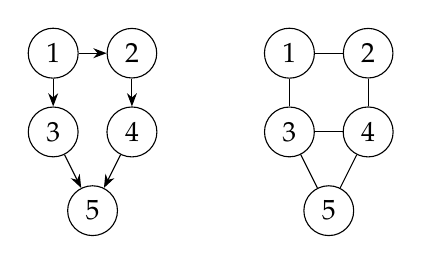
\begin{tikzpicture}
%\tikzstyle{place}=[circle,draw=blue!50,fill=blue!20,thick,inner sep=0pt,minimum size=6mm]
\begin{scope}[every node/.style={circle,draw}]
    \node (A) at (0,0) {$1$};
    \node (B) at (1,0) {$2$};
    \node (C) at (0,-1) {$3$};
    \node (D) at (1,-1) {$4$};
    \node (E) at (0.5,-2) {$5$};
    
    \node (F) at (3,0) {$1$};
    \node (G) at (4,0) {$2$};
    \node (H) at (3,-1) {$3$};
    \node (I) at (4,-1) {$4$};
    \node (J) at (3.5,-2) {$5$};
\end{scope}

\begin{scope}[>={Stealth[black]},
              every node/.style={fill=white,circle},
              every edge/.style={draw=black}]
    \path [->] (A) edge (B);
    \path [->] (A) edge (C);
    \path [->] (B) edge (D);
    \path [->] (C) edge (E);
    \path [->] (D) edge (E);
    
    \path [-] (F) edge (G);
    \path [-] (F) edge (H);
    \path [-] (G) edge (I);
    \path [-] (H) edge (I);
    \path [-] (H) edge (J);
    \path [-] (I) edge (J);
%    \path [-] (B) edge [bend right=60] (E); 
\end{scope}
\end{tikzpicture}
\caption{An example of a DAG whose moral graph is non-chordal.}
\end{figure}
For any given DAG $G$, it has a unique moral graph $F$ s.t. $B_V^G=B_V^F$. Figure \ref{fg:wrs_non_chordal} is an example of a DAG and its moral graph, which is non-choral. Hence, $\phi$ is non-surjective. \qed
\end{proof}


%\begin{figure}[H]
%  \centering
%    \includegraphics[scale=0.3]{wrs_non_chordal_example.png}
%  \caption{An example of a DAG whose moral graph is non-chordal.}
%  \label{fg:wrs_non_chordal}
%\end{figure}

\section{Weak recursively simplicial graphs}
\begin{definition}
\label{def:collider}
A \textbf{collider} in a hybrid graph is a node with at least two parents. 
\end{definition}

\begin{definition}
\label{def:consistent_ext}
A DAG $G$ is a \textbf{consistent extension} of a hybrid graph $H$ if $G$ and $H$ have the same skeleton and the same set of colliders. 
\end{definition}

Let $F=(V,E)$ be a graph over $n$ nodes. Let $S=\{S_1, \dots, S_m\}$ be a set of disjoint subsets of $V$ s.t. $\cup_{i=1}^m S_i=V$. Let $U=\{U_1, \dots, U_m\}$ be a set of disjoint subsets of $E$, where $U_i \subseteq \{v_jv_k \mid \forall v_j, v_k \in N_l, \forall v_l \in S_i\}$. Two extremes of $U_i$ are the empty set and the edges between all pairs of neighbours of $v_l$ for all $v_l \in S_i$. We use $O = \{(S_1, U_1), \dots, (S_m, U_m)\}$ to denote the pairs. Next we introduce a subset of undirected graphs which are not as strong as recusrively simplicial.  

\begin{definition}
\label{def:wrs}
A graph $F=(V,E)$ is \textbf{weak recursively simplicial (WRS)} if there exits $O = \{(S_1, U_1), \dots, (S_m, U_m)\}$ such that $S_1$ is the set of simplicial nodes in $F$ and $S_{i}$ is the set of simplicial nodes in the subgraph obtained by removing from $F$ the pairs $\{O_1, \dots, O_{i-1}\}$ for $i \in [2,m]$. 
\end{definition}
The reason such a graph is named weak recursively simplicial is because if we only remove the simplicial nodes from $F$, the induced subgraph over the remaining nodes may or may not have any simplicial nodes. So none or some edges between neighbours of simplicial nodes may need to be removed as well to retain the recursion. By definition, a chordal graph is also weak recursively simplicial by letting $U_i=\emptyset$. The converse, however, is not true. The graph on the right of Figure \ref{fg:wrs_non_chordal} is a WRS graph. It has $O_1 = \{S_1=\{5\}, U_1=\{3-4\}\}$. The subgraph obtained by removing $O_1$ is a chordal graph that is also WRS. Therefore, the original graph is WRS.  

\begin{theorem}
\label{prop:moral_implies_wrs}
Let $G=(V,E)$ be a DAG and $F$ be the moral graph of $G$. Then $F$ is weak recursively simplicial. 
\end{theorem}

\begin{proof}
(Base case) $G(1) = F(1)$ is a single node graph, so $F(1)$ is WRS. (Inductive hypothesis) Assuming the moral graph $F(n)$ of any DAG $G(n)$ with $n$ nodes is WRS. (Inductive step) Adding the node $v_{n+1}$ in $G(n)$ as a new leaf produces another DAG $G(n+1)$ with $n+1$ nodes. Since $v_{n+1}$ is a leaf in $G(n+1)$, it becomes a simplicial node in $F(n+1)$ after moralization. In addition, extra edges may be introduced to connect parents of $v_{n+1}$. Since $v_{n+1}$ is a simplicial node, it can be removed from $F(n+1)$ together with the extra edges introduced. Hence, we get back to the same moral graph $F(n)$ that is assumed to be WRS. Therefore, $F(n+1)$ is also WRS. \qed
\end{proof}
Theorem \ref{prop:moral_implies_wrs} suggests that the moral graph of any DAG is WRS. To prove there is a one-to-one correspondance between moral graphs and WRS graphs, we want to show that the converse is also true. That is, a WRS graph $F$ can be oriented into a DAG $G$ (possibly with some edge removal) such that the moral graph of $G$ is identical to $F$. 

\begin{theorem}
\label{prop:wrs_implies_moral}
Let $F=(V,E)$ be a weak recursively simplicial graph. Then $F$ is the moral graph of a DAG. 
\end{theorem}

\begin{proof}
(Base case) $F(1)$ is a single node WRS graph, and also the moral graph of the single node DAG $G(1)$. (Inductive hypothesis) Assuming any WRS graph $F(n)$ with $n$ nodes is the moral graph of a DAG $G(n)$. (Inductive step) Adding $v_{n+1}$ into $F(n)$ as a simplical node, so the resulting graph $F(n+1)$ is WRS. Since $v_{n+1}$ is a simplicial node, there exists a DAG $G(n+1)$, in which $v_{n+1}$ is a leaf. Therefore, the moral graph of $G(n+1)$ is $F(n+1)$. \qed

%$F$ is WRS implies the neighbours of a simplicial node in each  step can be directed towards the simplicial node. The resulting graph after recurtion is a hybrid graph $H$, the undirected edges in which are between neighbours of simplicial node. In addition, the two end nodes of any undirected edges must not be simplicial nodes. For otherwise, the edges would have been directed too. Therefore, $H$ must have a DAG extension $G$ which has the same skeleton and set of colliders as $H$. Since the edges removed are between spouses whose common child is a simplicial node, we have $B_G = B_F$. Therefore, $F$ is the moral graph of $G$. \qed
\end{proof}

\begin{corollary}
\label{cor:wrs_equal_moral}
An undirected graph is weak recursively simplicial if and only if it is the moral graph of a DAG. 
\end{corollary}
\begin{proof}
The corollary follows from the Theorem \ref{prop:moral_implies_wrs} and Theorem \ref{prop:wrs_implies_moral}. \qed
\end{proof}

\begin{corollary}
Let $\mathcal{F}=\{F=(V,E) \mid F \text{ is weak recursively simplicial}\}$ be the set of weak recursively simplicial graphs over $V$ and $\mathcal{B} = \{B_V^G \mid \text{for all DAG $G$ over $V$}\}$ be the set of Markov blanket families of any DAG over $V$. Then $|\mathcal{F}| = |\mathcal{B}|$. 
\end{corollary}
\begin{proof}
It is straightforward that there is a one-to-one correspondance between $\mathcal{B}$ and moral graphs. Hence, Corollary \ref{cor:wrs_equal_moral} implies that $\mathcal{F}$ has a one-to-one correspondance with $\mathcal{B}$, so equal cardinality. \qed
\end{proof}

Next, we present a backtracking algorithm for checking whether or not a given graph $F=(V,E)$ is WRS. If it is, the algorithm will find a DAG $G$, the moral graph of whom is $F$. Notice that this algorithm may produce a hybrid graph, which always has a consistent DAG extension according to Proposition \ref{prop:wrs_implies_moral}. Hence, we use the algorithm presented in \cite{dor1992simple} to get it. 
\begin{algorithm}[]
\caption{Backtracking algorithm to test WRS of graphs}
\label{alg:wrs_bktr}
\begin{algorithmic}[]
	\Require{$F$ is an undirected graph obtained by connecting all $v_j \in B_i$ with $v_j, \forall v_j \in V$}
    \Statex
    \Function{$WRS$}{$F$}
    \If{$F$ is chordal} 
    	\Return {TRUE} 
    \EndIf
    \State Find the set $S$ of all simplicial nodes in $F$
    \If{$S \neq \emptyset$} 
    	\State Find $E=\{v_jv_k \mid \forall v_j, v_k \in N_i, \forall v_i \in S\}$
    	\State $backup = F$
    	\ForEach{$U \subseteq E$} \Comment{for each subset of $E$}
    	\State $F=backup$
    	\State $F=F-S-U$ \Comment{Remove simplicial nodes $S$ and edges $U$}
        \If{$WRS(F)=$ TRUE}
        	\Return {TRUE}
        \EndIf
      \EndFor
    \EndIf
    \State \Return{FALSE}
    \EndFunction
\end{algorithmic}
\end{algorithm}


\section{Polytree}
\begin{proposition}
\label{prop:moral_of_pt_chordal}
Let $T=(V,E)$ be a polytree and $F$ be the moral graph of $T$. Then $F$ is a chordal graph. 
\end{proposition}
\begin{proof}
Assuming $F$ is not a chordal graph, there must exist a chordless $C_m \subset F$ for $m\ge 4$. $F$ being moral implies that the $C_m$ shares an edge with a simplicial clique $K_n$ for $n \ge 3$. Hence, there are multiple paths between a node in the $C_m$ and the simplicial node in the $K_n$ via different neighbours of the simplicial node. Henc, the assumption leads to a contradiction to $T$ being singly connected. \qed
\end{proof}

The converse of Proposition \ref{prop:moral_of_pt_chordal} is not true. For example, the chordal moral graph in Figure \ref{fg:chordal_over_4nodes} comes from a non-singly connected DAG. 
\begin{figure}[H]
\centering
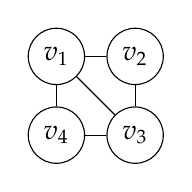
\begin{tikzpicture}
%\tikzstyle{place}=[circle,draw=blue!50,fill=blue!20,thick,inner sep=0pt,minimum size=6mm]
\begin{scope}[every node/.style={circle,draw}]           
    \node (A) at (2,2) {$v_1$};
    \node (B) at (3,2) {$v_2$};
    \node (C) at (3,1) {$v_3$};
    \node (D) at (2,1) {$v_4$};
    
    \path [-] (A) edge (B);
    \path [-] (A) edge (D);
    \path [-] (C) edge (D);
    \path [-] (C) edge (B);
    \path [-] (A) edge (C);
\end{scope}
\end{tikzpicture}
\caption{A chordal graph that comes from moralizing a non-singly connected DAG.}
\label{fg:chordal_over_4nodes}
\end{figure}

\begin{corollary}
Let $B_X$ be a set of Markov blankets over a variable set $X$. The problem of testing if $B_X$ is consistent with a polytree tree is in polynomial time.
\end{corollary}
\begin{proof}
Chordality can be verified in polynomial time (citation!!!). \qed
\end{proof}

\textbf{Idea:} Since it is in polynomial time to check if a set of learned $B_X$ is consistent with a DAG or not, we could start the structure discovery process by learning a polytree over all variables in $X$. Then gradually build up a DAG from a polytree. In addition, because a polytree is a subset of DAGs, so there would be less number of consistent polytrees to a chordal graph than consistent DAGs to a wrs graph.  

\section{Complexity}
\begin{definition}
Let $F=(V,E)$ be an undirected graph. A clique over a subset of variables $S \subset V$ is called a \textbf{simplicial clique} if $v_i \in S$ is a simplicial node in $F$. A \textbf{maximal simplicial clique} is a simplicial clique that cannot be extended by including one more vertex. 
\end{definition}
For example, $5-3$ and $5-4$ in Figure \ref{fg:envelope} are two simplicial cliques of size 2. The maximal simplicial clique is over nodes $\{3,4,5\}$.

WRS involves indefinite edge removal, depending on whether or not the induced subgraph obtained by removing a simplicial node is again WRS. Recursively simplicial is an extreme case of WRS where no edge is removed. In this section, we show that another extreme of WRS where a simplicial clique is always removed can be adopted to check morality for maximum degree $3$ graphs in polynomial time. 

\begin{theorem}
\label{thm:deg3}
Let $F=(V,E)$ be a connected moral graph with maximum degree $\Delta(F)=3$. Then the morality of $F$ can be checked by recursively removing a simplicial clique.
\end{theorem}
\begin{proof}
Assuming $F$ is a moral graph with $\Delta(F)=3$ and its morality cannot be checked by recursively removing a simplicial clique. It follows that the recursion must stop at a subgraph $F'' \subset F$ that has no simplicial nodes. $F$ is WRS and $\Delta(F)=3$ imply that $F''$ must share an edge with a $3$-clique $K_3$ (Figure \ref{fg:deg_3_dwrs}) that exists outside of $F''$ and will become simplicial during the recursive WRS process. $F''$ has no simplicial nodes implies that at least one of the two edges $\{v_5-v_3, v_5-v_4\}$ in $K_3$ must be removed during the recursive process of removing simplicial cliques. This requires $K_3$ to share an edge with another $k$-clique for $k\ge 3$. However, the nodes $v_3$ and $v_4$ have degree $3$ implies $K_3$ cannot share an edge with anything else. Hence, we reach a contradiction. \qed

%However, the degrees of nodes $v_3$ and $v_4$ have reached the maximum, hence no clique can be attached. Therefore there is a contradiction that $F$ being moral but not D-WRS. \qed
\end{proof}
\begin{figure}[H]
\centering
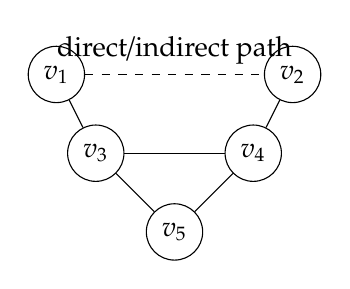
\begin{tikzpicture}
%\tikzstyle{place}=[circle,draw=blue!50,fill=blue!20,thick,inner sep=0pt,minimum size=6mm]
\begin{scope}[every node/.style={circle,draw}]           
    \node (A) at (2,2) {$v_1$};
    \node (B) at (5,2) {$v_2$};
    \node (C) at (2.5,1) {$v_3$};
    \node (D) at (4.5,1) {$v_4$};
    \node (E) at (3.5,0) {$v_5$};  
    
    \path [-] (A) edge (C);
    \path [-] (B) edge (D);
    \path [-] (C) edge (D);
    \path [-] (C) edge (E);
    \path [-] (D) edge (E);  
\end{scope}
	\draw [dashed] (A) -- (B) node[above,midway,sloped] {direct/indirect path};
\end{tikzpicture}
\caption{The subgraph $F''$ is over $\{v_1,v_2,v_3,v_4,\dots\}$, its supergraph $F'$ is over $\{v_1,v_2,v_3,v_4,v_5,\dots\}$.}
\label{fg:deg_3_dwrs}
\end{figure}

\begin{corollary}
The process of checking whether a given undirected graph $F$ with maximum degree $\Delta(F) \le 3$ is weak recursively simplicial is in polynomial time. 
\end{corollary}
\begin{proof}
The definite process of removing a simplicial clique takes the same time as just removing a simplicial node, hence it is in polynomial time. \qed 
\end{proof}

We first prove the following two lemmas that will be used to prove Theorem \ref{thm:deg4}. 
\begin{lemma}
\label{lm:long_stack}
Let $F=(V,E)$ be an undirected graph with maximum degree $\Delta(F)=4$. Let $S \subset F$ be an induced subgraph such that $S$ is a stack of at least 4 $K_3$s in a row (Figure \ref{fg:4k3s}). Assuming $v_1$ is a simplicial node in $F$, then $F$ is WRS if and only if $G=(V\setminus \{v_1\}, E\setminus \{v_1v_2,v_1v_3,v_2v_3\})$ is WRS. 
\begin{figure}[H]
\centering
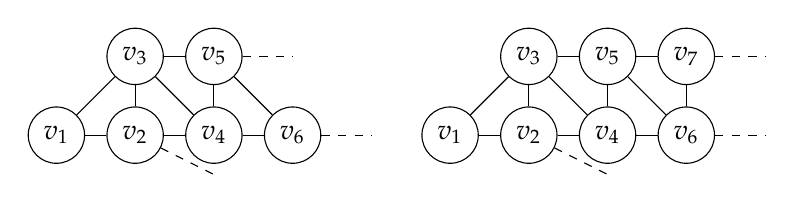
\begin{tikzpicture}
%\tikzstyle{place}=[circle,draw=blue!50,fill=blue!20,thick,inner sep=0pt,minimum size=6mm]
\begin{scope}[every node/.style={circle,draw}]               
    \node (a) at (0,0) {$v_1$};
    \node (b) at (1,0) {$v_2$};
    \node (c) at (1,1) {$v_3$};  
    \node (d) at (2,0) {$v_4$};
    \node (e) at (2,1) {$v_5$};
    \node (f) at (3,0) {$v_6$};
    \path [-] (a) edge (c);
    \path [-] (a) edge (b);
    \path [-] (b) edge (d);
    \path [-] (c) edge (b);
    \path [-] (c) edge (d);
    \path [-] (c) edge (e);
    \path [-] (d) edge (f); 
    \path [-] (d) edge (e);
    \path [-] (e) edge (f);
    \draw[dashed] (b) -- (2,-0.5);
    \draw[dashed] (e) -- (3,1);
    \draw[dashed] (f) -- (4,0); 
    
    \node (A) at (5,0) {$v_1$};
    \node (B) at (6,0) {$v_2$};
    \node (C) at (6,1) {$v_3$};  
    \node (D) at (7,0) {$v_4$};
    \node (E) at (7,1) {$v_5$};
    \node (F) at (8,1) {$v_7$};
    \node (G) at (8,0) {$v_6$};
    \path [-] (A) edge (C);
    \path [-] (A) edge (B);
    \path [-] (B) edge (D);
    \path [-] (C) edge (B);
    \path [-] (C) edge (D);
    \path [-] (C) edge (E);
    \path [-] (D) edge (E);
    \path [-] (E) edge (F);
    \path [-] (D) edge (G);
    \path [-] (F) edge (G);  
    \path [-] (E) edge (G);   
    \draw[dashed] (B) -- (7,-0.5);
    \draw[dashed] (G) -- (9,0);
    \draw[dashed] (F) -- (9,1);        
\end{scope}
\end{tikzpicture}
\caption{A stack of $4$ and $5$ $K_3$s is contained in a maximum degree $4$ graph $F$.}
\label{fg:4k3s}
\end{figure}
\end{lemma}
\begin{proof}
Figure \ref{fg:4k3s} shows a stack of four and five $K_3$s. In either case, the two nodes on each end have degrees less than $4$. Assuming $v_1$ is a simplicial node, the other three nodes can be adjacent to others nodes in $F$. Removing $v_1$ and the three edges in the simplicial clique, $v_3$ has degree $2$ hence is a simplicial node in $G$. Because $v_1$ is simplicial in $F$ and $d_F(v_3)=d_F(v_4)=4$, none of $\{v_1,v_3,v_4\}$ is adjancent to any nodes in $F$ other than their neighbours in $S$. Hence, the two cliques over $\{v_1,v_2,v_3\}$ and $\{v_2,v_3,v_4\}$ are not necessary breakers for any cycle in $F$. In addition, the process of removing the simplical $K_3$ does not break more cliques. Hence, if $F$ is WRS then $G$ is also WRS. The argument can be extend to $S$ with arbitrary (even or odd) number of $K_3$s. 

The only if condition is obvious. If $G$ is WRS, the new graph $F$ obtained by attaching a simplcial $K_3$ to $G$ is still WRS. \qed
\end{proof}


\begin{lemma}
\label{lm:2k3s}
Let $F=(V,E)$ be an undirected graph with maximum degree $\Delta(F)=4$. Let $S\subset F$ be an induced subgraph such that $S$ is a stack of two $K_3$s (Figure \ref{fg:2k3s}). Assuming $v_1$ is a simplicial node, then $F$ is WRS i$G=(V\setminus \{v_1\},E\setminus \{v_1v_2,v_1v_3\})$ is WRS.
\begin{figure}[H]
\centering
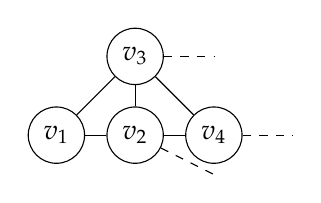
\begin{tikzpicture}
%\tikzstyle{place}=[circle,draw=blue!50,fill=blue!20,thick,inner sep=0pt,minimum size=6mm]
\begin{scope}[every node/.style={circle,draw}]               
    \node (a) at (0,0) {$v_1$};
    \node (b) at (1,0) {$v_2$};
    \node (c) at (1,1) {$v_3$};  
    \node (d) at (2,0) {$v_4$};
        
    \path [-] (a) edge (c);
    \path [-] (a) edge (b);
    \path [-] (b) edge (d);
    \path [-] (c) edge (b);
    \path [-] (c) edge (d);
    \draw[dashed] (b) -- (2,-0.5);
    \draw[dashed] (c) -- (2,1);
    \draw[dashed] (d) -- (3,0);        
\end{scope}
\end{tikzpicture}
\caption{A stack of 2 $K_3$s is contained in a maximum degree $4$ graph $F$.}
\label{fg:2k3s}
\end{figure}
\end{lemma}
\begin{proof}
Since $v_1$ is a simplicial node with degree $2$, it is not adjacent to any nodes other than $\{v_2,v_3\}$. Hence, the simplicial clique is not a necessary breaker for any cycle in $F$. In addition, the process of removing $\{v_1, v_1v_2,v_1v_3\}$ does not reduce any simplicial clique in $F$. Hence, $G$ is still WRS. If $G$ is WRS, $F$ is different from $G$ by a simplcial node $v_1$, so $F$ is also WRS. \qed
\end{proof}

It is worth noticing that if $S$ is a stack of $3$ $K_3$s, there is no universal answer for all conditions. Hence, the following theorem states a set of rules for different sinarios and proves that the rules are legitimate for checking morality of maximum degree $4$ graphs. 
\begin{figure}[H]
\centering
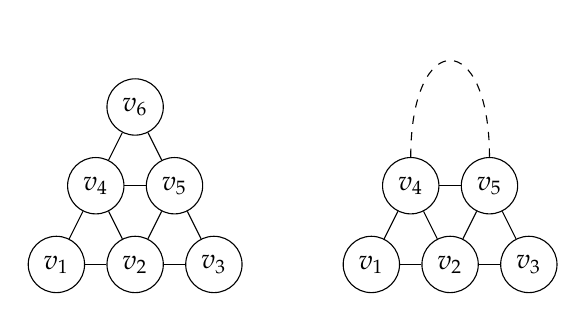
\begin{tikzpicture}
\begin{scope}[every node/.style={circle,draw}] 
	\node (A) at (3.5,-2) {$v_1$};
    \node (B) at (5.5,-2) {$v_3$};
    \node (F) at (4.5,0) {$v_6$};
    \node (H) at (4,-1) {$v_4$};
    \node (I) at (5,-1) {$v_5$};
    \node (J) at (4.5,-2) {$v_2$};
         
    \node (a) at (7.5,-2) {$v_1$};
    \node (b) at (9.5,-2) {$v_3$};
    %\node (f) at (8,0) {$v_6$};
    %\node (g) at (9,0) {$v_7$};
    \node (h) at (8,-1) {$v_4$};
    \node (i) at (9,-1) {$v_5$};
    \node (j) at (8.5,-2) {$v_2$};
\end{scope}

\begin{scope}[>={Stealth[black]},
              every node/.style={fill=white,circle},
              every edge/.style={draw=black}] 
              
    \path [-] (A) edge (J);
    \path [-] (A) edge (H);
    \path [-] (B) edge (I);
    \path [-] (B) edge (J);
    \path [-] (F) edge (H);
    \path [-] (F) edge (I);
    \path [-] (H) edge (I);
    \path [-] (H) edge (J);
    \path [-] (I) edge (J);
                     
    \path [-] (a) edge (j);
    \path [-] (a) edge (h);
    \path [-] (b) edge (i);
    \path [-] (b) edge (j);
    %\path [-] (f) edge (g);
    %\path [-] (f) edge (h);
    %\path [-] (g) edge (i);
    \path [-] (h) edge (i);
    \path [-] (h) edge (j);
    \path [-] (i) edge (j);
%    \path [-] (B) edge [bend right=60] (E); 
\end{scope}
\draw[dashed] (h) .. controls (8,1) and (9,1) .. (i);
\end{tikzpicture}
\caption{Two graphs $G_1$ (left) and $G_2$ (right) of maximum degree $4$. The dashed line represents a path of length at least $3$.}
\label{fg:special_graphs}
\end{figure}

\textcolor{red}{all graphs are assumed to be connected. Denote a simplicial $K_4$ with the simplicial node $s$ by $K_4^s$.}

\begin{algorithm}[]
\caption{Backtracking algorithm to test WRS of graphs}
\label{alg:wrs_bktr}
\begin{algorithmic}[]
	\Require{an undirected graph $F=(V,E)$ s.t. $\Delta(F)=4$}
    \Statex
    \Function{$\phi$}{$F$}
    \If{$F$ is chordal} 
    	\Return {TRUE} 
    \EndIf
    
	\State Find the set $S$ of all simplicial nodes in $F$
	\State Order $S$ by nodes degree $\{0, 1, 3, 2\}$
	\State For degree $2$ nodes $x, y \in S$, if $y \in G_2$ whilest $x \notin G_2$, $I(x) < I(y)$
	\State $s = S[1]$
	
    \If{$d(s)\le 1$} \Comment{0. Prune all leaves}
    	\State{$F=F[V\setminus \{s\}]$}
    	\If{$\phi(F)=$ TRUE}
        	\Return {TRUE}
        \EndIf
        \State \Return {FALSE} 
    \EndIf

    \If{$d(s)=3$} \Comment{1. Remove simplicial $K_4$}
    	\State{$F=F-K_4^s$}
    	\If{$\phi(F)=$ TRUE}
        	\Return {TRUE}
        \EndIf
    \State \Return {FALSE}        
    \EndIf
    
    \If{$d(s)=2$} \Comment{2. For a simplicial $K_3$}
    	\If{$\phi(F)=$ TRUE}
        	\Return {TRUE}
        \EndIf
        \State \Return {FALSE} 
    \EndIf
    
    	
    \State \Return{FALSE}
    \EndFunction
\end{algorithmic}
\end{algorithm}

\begin{theorem}
\label{thm:deg4}
Let $F=(V,E)$ be an undirected graph with maximum degree $\Delta(F)=4$. Let $O_1$ and $O_2$ denote the operations of removing a simplicial node and a simplicial clique respectively. Then the morality of $F$ can be checked by the following steps:
\begin{enumerate}
\item If seeing a simplicial $K_4$ or $K_5$, apply $O_2$.
\item If a simplicial $K_3$, 
\begin{enumerate}
\item shares an edge with a $K_4$, apply $O_1$;
\item forms a subgraph with three other $K_3$s as shown in Figure \ref{fg:special_graphs} left, apply $O_2$;
\item is in a stack of one or more than three $K_3$s, apply $O_2$;
\item is in a stack of two $K_3$s, apply $O_1$;
\item is in a stack of three $K_3$s, 
\begin{enumerate}
\item if it is not in a subgraph as shown in Figure \ref{fg:special_graphs} right, apply $O_2$;
\item if all simplicial nodes are in subgraphs as shown in Figure \ref{fg:special_graphs} right, 
\begin{enumerate}
\item if two simplicial nodes are in the same stack of $K_3$s, apply $O_1$ on both;
\item if no two simplicial nodes are in the same stack of $K_3$s, apply $O_2$ on a random simplicial node.  
\end{enumerate}
\end{enumerate}
\end{enumerate}
\end{enumerate}
\end{theorem}

%When checking morality of an undirected graph $F$ using backtracking, the indefinite edge removals sometimes lead a search to a dead end. So the search backtracks to the most recent state where there are multiple options and takes the next unchecked option. The risk of indefinite edge removal is that it may delete an edge from a clique that is necessary for breaking a cycle in $F$ (Figure \ref{fg:special_graphs} right). This, however, is not a problem if a simplicial clique shares an edge with only incomplete subgraphs such as tree or cycle, because in such cases an edge can be deleted without causing problems (Figure \ref{fg:sn_with_incomplete} left). To prove the above theorem, we only consider the cases when a simplicial clique shares an edge with a complete subgraph. 

\begin{proof}
The maximum degree $\Delta(F)=4$ implies that a simplicial clique $S=K_m$ where $1 \le m \le 5$. For $m=\{1,2\}$, the cases are trivial so we simply prune the simplicial node of $S$. For $m=5$, each node of a $K_5$ has degree 4 so a $K_5$ is either a (connect) component of $F$ or it is $F$. In either case, a $K_5$ can be removed completely. 

When $m=4$, each node in a $K_4$ has degree $3$. One node is reserved for a simplicial node, so only one edge can be shared with a complete subgraph $K_3$ (Figure \ref{fg:k4+k3}). Since two nodes $\{v_2,v_4\}$ reach the maximum degree, none of the three edges of the $K_3$ appears in a \textbf{simple cycle} that shares no edge with the $K_4$. Equivalently, if the simplicial node $v_1$ and the two edges $\{v_2v_3,v_3v_4\}$ are removed, the $K_3$ shares no edges with a simple cycle in the remaining graph. Hence, the simplicail $K_4$ can be removed completely. 
\begin{figure}[H]
\centering
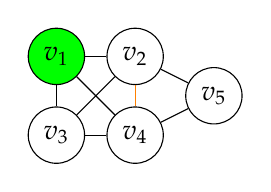
\begin{tikzpicture}
%\tikzstyle{place}=[circle,draw=blue!50,fill=blue!20,thick,inner sep=0pt,minimum size=6mm]
\begin{scope}[every node/.style={circle,draw}]               
    \node (a) at (9,0.5) {$v_5$};
    \node[fill=green] (c) at (7,1) {$v_1$};
    \node (d) at (8,1) {$v_2$};
    \node (e) at (7,0) {$v_3$};  
    \node (f) at (8,0) {$v_4$};
    
    \path [-] (a) edge (d);
    \path [-] (a) edge (f);
    \path [-] (c) edge (d);
    \path [-] (c) edge (e);
    \path [-] (d) edge (e); 
    \path [-] (c) edge (f);
    \path [-] (d) edge (f); 
    \path [-] (e) edge (f);
\end{scope}
	\draw [orange] (d) -- (f);
\end{tikzpicture}
\caption{A simplicial $K_4$ over $\{v_1,v_2,v_3,v_4\}$ shares an edge $v_2v_4$ with a $K_3$ over $\{v_2,v_4,v_5\}$.}
\label{fg:k4+k3}
\end{figure}

When $m=3$, each node in a $K_3$ has degree 2. Researve one node as the simplicial node leaves only one edge free to be shared with subgraphs of $F$. Denote the free edge by $e$. If $e=K_3 \cap K_4$, remove the simplicial node of the $K_3$ leads to the case of seeing a simplicial $K_4$ that has been proved above. If $e=K_3\cap K_3$, each of $e$'s end node has degree $3$ hence opens more possibilities. By Lemma \ref{lm:2k3s}, ...



Assuming there is a stack of even number of $K_3$s, then only four nodes $\{v_1,v_2,v_5,v_6\}$ have degree less than $4$. If one of the end node is reserved as a simplicial node, 
\begin{figure}[H]
\centering
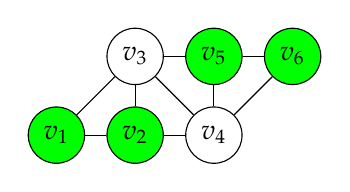
\begin{tikzpicture}
%\tikzstyle{place}=[circle,draw=blue!50,fill=blue!20,thick,inner sep=0pt,minimum size=6mm]
\begin{scope}[every node/.style={circle,draw}]               
    \node[fill=green] (a) at (0,0) {$v_1$};
    \node[fill=green] (b) at (1,0) {$v_2$};
    \node (c) at (1,1) {$v_3$};  
    \node (d) at (2,0) {$v_4$};
    \node[fill=green] (e) at (2,1) {$v_5$};
    \node[fill=green] (f) at (3,1) {$v_6$};
    
    \path [-] (a) edge (c);
    \path [-] (a) edge (b);
    \path [-] (b) edge (d);
    \path [-] (c) edge (b);
    \path [-] (c) edge (d);
    \path [-] (c) edge (e);
    \path [-] (d) edge (f); 
    \path [-] (d) edge (e);
    \path [-] (e) edge (f);
\end{scope}
\end{tikzpicture}
%\caption{A simplicial $K_4$ over $\{v_1,v_2,v_3,v_4\}$ shares an edge with a $K_3$ over $\{v_2,v_4,v_5\}$.}
%\label{fg:k4+k3}
\end{figure}



\underline{$K_3+\{K_3,K_3\}$:} The edge $v_2-v_3$ is shared by three $K_3$s (Figure \ref{fg:k3+} bottom right). If the simplicial $K_3$ is removed, the remaining two $K_3$s form a $C_4$. Since the nodes $\{v_2,v_3\}$ reach the maximum degree and are not adjacent to each other, the $C_4$ cannot share an edge with another $K_3$. The graph will then be falsely classified as non-WRS. Hence, only the simplicial node is removed in this case.  

\underline{$K_3+\{K_3,C_m\}$:} If the simplicial node $v_1$ is removed (Figure \ref{fg:k3+} bottom left), the remaining $K_3$ over $\{v_2,v_3,v_4\}$ becomes a potential breaker for the $C_m$, although other breakers may exist for the same cycle. 
\end{proof}



\cite{verma1993deciding} proved that the problem of deciding whether an undirected graph is WRS is NP-complete. We modifed the prove so that the NP-completeness hodes for undirected graphs with maximum degree 5. 
\begin{proposition}
The problem of testing whether a given undirected graph with maximum degree 5 is weak recursively simplicial is NP-complete. 
\end{proposition}

\begin{proof}
Replace the arbitrarily high degree nodes with chains. Figures!!! \qed
\end{proof} 


\iffalse
\newpage
\begin{figure}
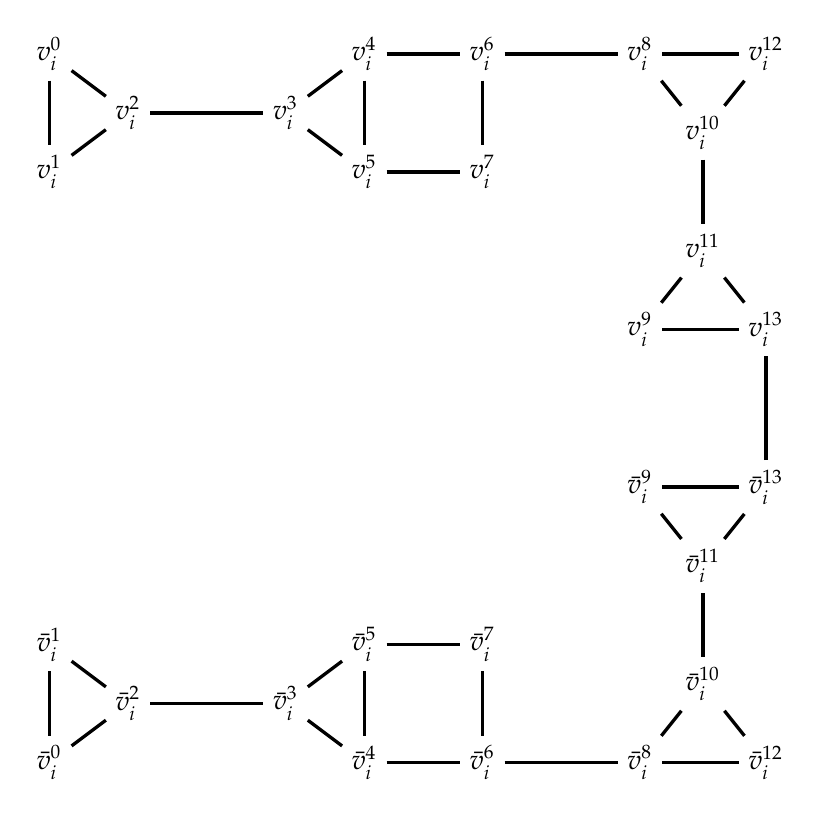
\begin{tikzpicture}
%\tikzstyle{place}=[circle,draw=blue!50,fill=blue!20,thick,inner sep=0pt,minimum size=6mm]
%\begin{scope}[every node/.style={circle,thick,draw,minimum size=3mm}]
\begin{scope}
    \node (A) at (0,0) {$v_i^0$};
    \node (B) at (0,-1.5) {$v_i^1$};
    \node (C) at (1,-0.75) {$v_i^2$};
    \node (D) at (3,-0.75) {$v_i^3$};
    \node (E) at (4,0) {$v_i^4$};
    \node (F) at (4,-1.5) {$v_i^5$};
    \node (G) at (5.5,0) {$v_i^6$};
    \node (H) at (5.5,-1.5) {$v_i^7$};
    \node (I) at (7.5,0) {$v_i^8$};
    \node (J) at (9.1,0) {$v_i^{12}$};
    \node (K) at (8.3,-1) {$v_i^{10}$};
    \node (L) at (8.3,-2.5) {$v_i^{11}$};
    \node (M) at (7.5,-3.5) {$v_i^{9}$};
    \node (N) at (9.1,-3.5) {$v_i^{13}$};
    
    \node (O) at (0,-7.5) {$\bar{v}_i^1$};
    \node (P) at (0,-9) {$\bar{v}_i^0$};
    \node (Q) at (1,-8.25) {$\bar{v}_i^2$};
    \node (R) at (3,-8.25) {$\bar{v}_i^3$};
    \node (S) at (4,-7.5) {$\bar{v}_i^5$};
    \node (T) at (4,-9) {$\bar{v}_i^4$};
    \node (U) at (5.5,-7.5) {$\bar{v}_i^7$};
    \node (V) at (5.5,-9) {$\bar{v}_i^6$};
    \node (W) at (7.5,-9) {$\bar{v}_i^8$};
    \node (X) at (9.1,-9) {$\bar{v}_i^{12}$};
    \node (Y) at (8.3,-8) {$\bar{v}_i^{10}$};
    \node (Z) at (8.3,-6.5) {$\bar{v}_i^{11}$};
    \node (a) at (7.5,-5.5) {$\bar{v}_i^{9}$};
    \node (b) at (9.1,-5.5) {$\bar{v}_i^{13}$};
\end{scope}

\begin{scope}[>={Stealth[black]},
              every node/.style={fill=white,circle},
              every edge/.style={draw=black,very thick}]
    \path [-] (A) edge (B);
    \path [-] (A) edge (C);
    \path [-] (B) edge (C);
    \path [-] (C) edge (D);
    \path [-] (D) edge (E);
    \path [-] (D) edge (F);
    \path [-] (E) edge (F);
    \path [-] (E) edge (G);
    \path [-] (F) edge (H);
    \path [-] (G) edge (H);
    \path [-] (G) edge (I);
    \path [-] (I) edge (J);
    \path [-] (I) edge (K);
    \path [-] (J) edge (K);
    \path [-] (K) edge (L);
    \path [-] (L) edge (M);
    \path [-] (L) edge (N);
    \path [-] (M) edge (N);
    
    \path [-] (O) edge (P);
    \path [-] (O) edge (Q);
    \path [-] (P) edge (Q);
    \path [-] (Q) edge (R);
    \path [-] (R) edge (S);
    \path [-] (R) edge (T);
    \path [-] (S) edge (T);
    \path [-] (S) edge (U);
    \path [-] (T) edge (V);
    \path [-] (U) edge (V);
    \path [-] (V) edge (W);
    \path [-] (W) edge (X);
    \path [-] (X) edge (Y);
    \path [-] (W) edge (Y);
    \path [-] (Y) edge (Z);
    \path [-] (Z) edge (a);
    \path [-] (Z) edge (b);
    \path [-] (a) edge (b);
    
    \path [-] (b) edge (N);
%    \path [-] (B) edge [bend right=60] (E); 
\end{scope}
\end{tikzpicture}
\caption{A variable gedget, where the upper half corrsponds to the positive literal and the lower half corresponds to the negative literal.}
\end{figure}
\fi

\iffalse
\section{Unique prime decomposition}
The concept of simplicial decomposition of graphs was discussed by \cite{wagner1937eigenschaft}, \cite{halin1964simpliziale}, and \cite{diestel1987simplicial}. One of the important proofs is that any finite graphs (don't care about infinite graphs) has a prime decomposition, and such prime decomposition is unique. 
\fi

\section{Some random notes}
\begin{proposition}
Let $F$ be a moral 
\end{proposition}

\begin{figure}[H]
\centering
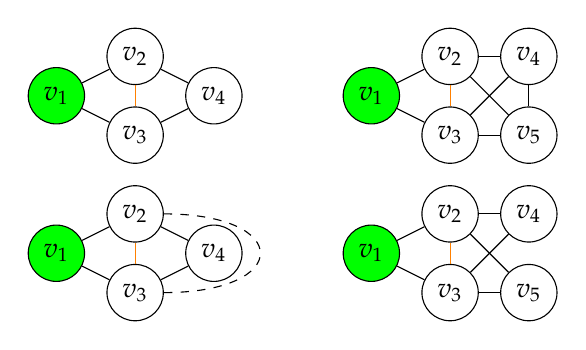
\begin{tikzpicture}
\begin{scope}[every node/.style={circle,draw}]               
	%k3+k3    
    \node[fill=green] (a) at (0,1) {$v_1$};
 	\node (b) at (1,1.5) {$v_2$};
 	\node (c) at (1,0.5) {$v_3$};
 	\node (d) at (2,1) {$v_4$};
    \path [-] (a) edge (b);
    \path [-] (a) edge (c);
    \draw[orange] (c) -- (b);        
    \path [-] (c) edge (d);
    \path [-] (b) edge (d);
    %k3+k4
    \node[fill=green] (aa) at (4,1) {$v_1$};
 	\node (bb) at (5,1.5) {$v_2$};
 	\node (cc) at (5,0.5) {$v_3$};
 	\node (dd) at (6,1.5) {$v_4$};
 	\node (ee) at (6, 0.5) {$v_5$};
    \path [-] (aa) edge (bb);
    \path [-] (aa) edge (cc);
    \draw[orange] (cc) -- (bb);        
    \path [-] (bb) edge (dd);
    \path [-] (cc) edge (ee);
    \path [-] (dd) edge (ee);
    \path [-] (dd) edge (cc);
    \path [-] (bb) edge (ee);   
    %k3+(k3+cm)
    \node[fill=green] (A) at (0,-1) {$v_1$};
 	\node (B) at (1,-0.5) {$v_2$};
 	\node (C) at (1,-1.5) {$v_3$};
 	\node (D) at (2,-1) {$v_4$};
    \path [-] (A) edge (B);
    \path [-] (A) edge (C);
    \draw[orange] (C) -- (B);     
    \path [-] (C) edge (D);
    \path [-] (B) edge (D);
    %k3+(k3+k3)
    \node[fill=green] (AA) at (4,-1) {$v_1$};
 	\node (BB) at (5,-0.5) {$v_2$};
 	\node (CC) at (5,-1.5) {$v_3$};
 	\node (DD) at (6,-0.5) {$v_4$};
 	\node (EE) at (6,-1.5) {$v_5$};
    \path [-] (AA) edge (BB);
    \path [-] (AA) edge (CC);
    \draw[orange] (CC) -- (BB);        
    \path [-] (CC) edge (DD);
    \path [-] (BB) edge (DD);
    \path [-] (BB) edge (EE);
    \path [-] (CC) edge (EE);        
    
\end{scope}
	\draw[dashed] (B) .. controls (3,-0.5) and (3,-1.5) .. (C);
\end{tikzpicture}
\caption{A simplicial $K_3$ over $\{v_1,v_2,v_3\}$ shares an edge with a $K_3$ (top left), $K_4$ (top right), $\{K_3, C_m\}$ (bottom left) or $\{K_3,K_3\}$ (bottom right).}
\label{fg:k3+}
\end{figure} 

\textbf{Lloyd's conjecture:} knowing a graph is wrs, adding an edge to obtain a supergraph, perhaps it is efficient to check if the supergraph is wrs.

\begin{proof}
because remove the added edge, then we obtain the original graph which we know is wrs. however, we don't remove a random edge when checking wrs unless the edge connects to a simplicial node. what if the edge is not connected with a sim node? if we know the original graph is wrs and we know the set of sim nodes in the recursion and the set of edges to delete, then we could easily check if the new edge is connected with any one of the sim node, if it is then good. if not, then we could check if the new edge is connected with two neighbours of a sim node, if it is then good. if a graph is wrs, then it eventually will diminish, so the new edge must appear somewhere in the recursion to either stop the recursion or don't stop it.
\end{proof} 

\begin{corollary}
DAGs in the same Markov equivalent class produce the same Markov blanket sets $B_X$. 
\end{corollary}
\begin{proof}
If two DAGs $G_1$ and $G_2$ are Markov equivalent, they have the same skeleton and the same set of colliders. This implies $B_i^{G_1} = B_i^{G_2}, \forall X_i \in X$. \qed
\end{proof}
Notice that two Markov equivalent classes could entail the same $B_X$. For example... 

\begin{corollary}
$|\{\text{chordal graphs}\}| \le |B_X| \le |\{\text{Markov equivalent classes}\}|$.
\end{corollary} 

Counting labelled chordal graphs \cite{wormald1985counting}, counting Markov equivalent classes (assymptotic ratio of around 0.27 to DAGs) \cite{gillispie2001enumerating}. 

\begin{table}[]
\centering
\caption{Comparison between the number of labelled connected chordal graphs, the number of weak recursively simplicial graphs, the number of undirected graphs and the number of Markov equivalent classes.}
\label{my-label}
\begin{tabular}{llllll}
\# nodes & \# con-C.G. & \# C.G. & \# WRS & \# U.G. & \# MEC \\ \hline
1        & 1& 1                 & 1          & 1         & 1 \\
2        & 1 & 2                 & 2          & 2         & 2 \\
3        & 4 & 8                 & 8          & 8         & 11 \\
4        & 35 & 61                & 61         & 64         & 185 \\
5        & 541 & 822               & 882        & 1024            & 8782\\
6        & 13302 & 18154             &       & 32768              & 1067825\\
7        & 489287 & 617675            &            & 2097152         & 312510571\\
8        & 25864897 & 30888596          &            &  268435456        & 212133402500 \\
9        & 1910753782 & 2192816760        &            &  68719476736       & 326266056291213 \\ 
10       & $1.93 \times 10^{11}$ & $2.15 \times 10^{11}$     &            & $3.52 \times 10^{13}$  & $1.19\times 10^{17}$ \\ \hline
\end{tabular}
\end{table}

\begin{proposition}
\label{prop:leaf_is_sim}
Let $G$ be a DAG and $F$ be the moral graph of $G$. If a node $x$ is a leaf in $G$, then it must be a simplicial node in $F$. 
\end{proposition}
\begin{proof}
If $x$ is a leaf in $G$, it has only parents, which form a clique after moralization. By definition, $x$ is a simplicial node in $F$. \qed
\end{proof}

\begin{corollary}
Let $G$ be a DAG and $F$ be the moral graph of $G$. Then $F$ must have at least one simplicial node. 
\end{corollary}

\begin{proof}
Since each DAG has at least one leaf, by Proposition \ref{prop:leaf_is_sim} $F$ have at least one simplicial node. \qed
\end{proof}

\begin{corollary}
\label{cor:negation_of_leaf_is_sim}
Let $G$ be a DAG and $F$ be the moral graph of $G$. If a node $x$ is not a simplicial node in $F$, then it must not be a leaf in $G$. 
\end{corollary}

\begin{proposition}
Let $G$ be a DAG and $F$ be the moral graph of $G$. Let $S^1$ be the set of simplicial nodes in $F$ and $F_1$ be the induced subgraph of $F$ over $X\setminus S^1$. Then there must exist at least one simplicial node after removing from $F'$ all the edges between $N(X_i), \forall X_i \in S^1$.
\end{proposition}

\begin{proof}
Let $F_1'$ be the result of removing from $F_1$ all the edges between $N(X_i), \forall X_i \in S^1$. The corresponding directed graph $G'$ of $F_1'$ must be a subgraph of the DAG $G$, so also acyclic. Assuming $F_1'$ has no simplicial nodes, by Corollary \ref{cor:negation_of_leaf_is_sim} $G'$ has no leaf, which is a contradiction. \qed
\end{proof}


Here are some issues worth discussing:
\begin{enumerate}
\item Application: the backtracking algorithm can now be applied when learning MBs in paralle. What if there are conflicts between two MBs, which one should give up? Need to estimate uncertainty?
\item Simplicial nodes in the first step always contain the leaves.
\item Those nodes that become simplicial in the next step without having to delete any edges contain the leaves in the next step. 
\item So wrs can be used to test if a MB family is consistent with a DAG, it would be good if we can also find out how many consistent DAGs or essential graphs are there for this MB family. 
\item also it would be good if we can explore wrs into details, such as what dag nodes become simplicial nodes in wrs recursion, and if no edges need to be deleted from a simplicial node's neighbours then what's this simplicial node?
\item maybe there is a path from s.t. every step is a moral graph of a dag, perhaps can be proved by delete an edge from a dag.   
\end{enumerate}

\textbf{Questions:} If a graph $F$ is known to be wrs, does is help to decide if a subgraph/supergraph different by one edge from $F$ is wrs or not?

\textbf{Answer:} Probably not. If it is, then we know a base case, any graph can be reached from this base case, hence any graph can be efficiently tested. 

\iffalse
The undirected edge connects two parents of a common child is called a \textit{moralized edge}. The process of obtaining a moral graph from a DAG is called \textit{moralization}. There is a unique moral graph of each DAG. Next, we define the reverse of a moralization process as \textit{demoralization}. It is defined on undirected graphs with at least one simplicial node. 
\fi

% the next proposition may not be true, so we omit it.
\iffalse
The next proposition proves that a chordal graph is also D-WRS, but not vice versa. 
\begin{proposition}
\label{prop:chordal_is_dwrs}
If $F=(V,E)$ is a chordal graph, then it is D-WRS. 
\end{proposition}
\begin{proof}
Assuming $F$ is not D-WRS. Then there is a subgraph $F' \subset F$ obtained by recursively remvoing all simplicial cliques from $F$ s.t. $F'$ has no simplicial clique. Hence, $F'$ must be cyclic 
\end{proof}


\begin{proof}
Being chordal is equivalent as being triangulated. If $F$ is chordal (Figure \ref{fg:chordal_is_dwrs}), removing the maximal simplicial clique of size 3 results in a subgraph of $F$ that has a maximal simplicial clique of size 2. Removing the size 2 maximal simplicial clique, we obtain a subgraph  that could also be obtained by recursively simplicial. \qed
\end{proof}
\begin{figure}[H]
\centering
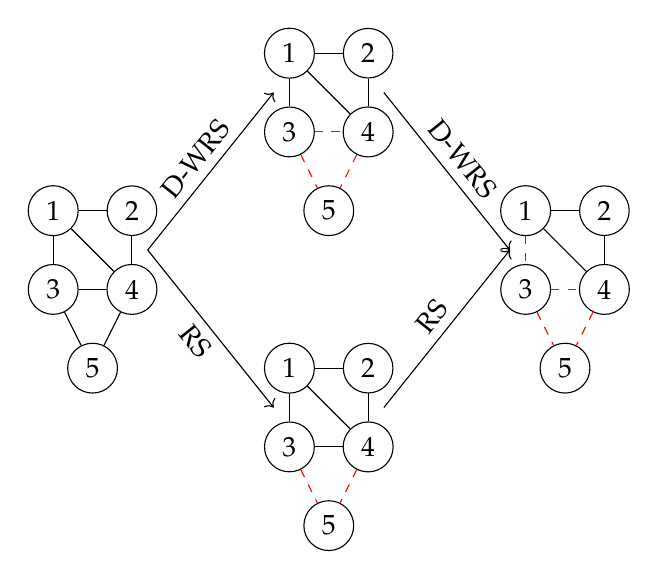
\begin{tikzpicture}
%\tikzstyle{place}=[circle,draw=blue!50,fill=blue!20,thick,inner sep=0pt,minimum size=6mm]
\begin{scope}[every node/.style={circle,draw}]  
    \node (F) at (0,0) {$1$};
    \node (G) at (1,0) {$2$};
    \node (H) at (0,-1) {$3$};
    \node (I) at (1,-1) {$4$};
    \node (J) at (0.5,-2) {$5$};
     
    \node (A) at (3,2) {$1$};
    \node (B) at (4,2) {$2$};
    \node (C) at (3,1) {$3$};
    \node (D) at (4,1) {$4$};
    \node (E) at (3.5,0) {$5$};
    
    \node (a) at (3,-2) {$1$};
    \node (b) at (4,-2) {$2$};
    \node (c) at (3,-3) {$3$};
    \node (d) at (4,-3) {$4$};
    \node (e) at (3.5,-4) {$5$};
    
    \node (K) at (6,0) {$1$};
    \node (L) at (7,0) {$2$};
    \node (M) at (6,-1) {$3$};
    \node (N) at (7,-1) {$4$};
    \node (O) at (6.5,-2) {$5$};
\end{scope}

\begin{scope}[>={Stealth[black]}]    
    \path [-] (F) edge (G);
    \path [-] (F) edge (H);
    \path [-] (G) edge (I);
    \path [-] (H) edge (I);
    \path [-] (H) edge (J);
    \path [-] (I) edge (J);
    \path [-] (F) edge (I);
        
    \path [-] (A) edge (B);
    \path [-] (A) edge (C);
    \path [-] (B) edge (D);
    \path [color=red,dashed] [-] (C) edge (D);
    \path [color=red,dashed][-] (C) edge (E);
    \path [color=red,dashed][-] (D) edge (E);
    \path [-] (A) edge (D);
    
    \path [-] (a) edge (b);
    \path [-] (a) edge (c);
    \path [-] (b) edge (d);
    \path [-] (c) edge (d);
    \path [color=red,dashed][-] (c) edge (e);
    \path [color=red,dashed][-] (d) edge (e);
    \path [-] (a) edge (d);
    
    \path [-] (K) edge (L);
    \path [color=red,dashed][-] (K) edge (M);
    \path [-] (L) edge (N);
    \path [color=red,dashed][-] (M) edge (N);
    \path [color=red,dashed][-] (M) edge (O);
    \path [color=red,dashed][-] (N) edge (O);
    \path [-] (K) edge (N);
\end{scope}

\begin{scope}[->,every node/.style={midway,sloped}]
	\draw (1.2,-0.5) -- (2.8,1.5) node[above] {D-WRS};
	\draw (1.2,-0.5) -- (2.8,-2.5) node[below] {RS};
    \draw (4.2,1.5) -- (5.8,-0.5) node[above] {D-WRS};
	\draw (4.2,-2.5) -- (5.8,-0.5) node[above] {RS};
\end{scope}	
\end{tikzpicture}
\caption{An example of a chordal graph is also D-WRS.}
\label{fg:chordal_is_dwrs}
\end{figure}

The converse of this proposition is not necessarily true (e.g., Figure \ref{fg:envelope}). If $F$ is a moral graph s.t. $\Delta(F) \le 2$, then F must be a tree hence chordal. By Proposition \ref{prop:chordal_is_dwrs} it must be D-WRS too. Next, we prove that $F$ is also D-WRS if $\Delta(F)=3$.
\fi

\section{Notations}
\subsection{Notations}
\begin{table}[]
\centering
\caption{Notations}
\label{my-label}
\begin{tabular}{ll}
\hline
$F$ &  a undirected graph \\
$G$ & a DAG \\
$X$ & a set of random variables (nodes) \\
$X_i$ & a random variable (or node) in $X$ \\
$X_{-i}$ & $X \setminus X_i$ \\ 
$X_{-[1,\dots, i]}$ & $X \setminus \{X_1, \dots, X_i\}$ \\ 
$B_i^G$ & the Markov blanket of a variable $X_i$ in $G$ \\ 
$B_X^G$ & $\{B_i \mid \forall X_i \in X\}$ \\ \hline
\end{tabular}
\end{table}

\bibliographystyle{named}
\bibliography{/home/kl/Documents/causal_discovery_ref_list}

\end{document}